\chapter{Methodology}

In this section, the nature of the data sets, the software tools that we used, and how the predictive models are going to be evaluated.

\section{Descriptions of Data}
Data sets to be analysed were the output of quartus OpenCL compiler. Data in each file can be categorised into three sections: pragma values, estimated resource usage summary and the detailed resource usage. Figure \ref{figure:sample_raw_data} is an instance of the data set.

\begin{figure}[h!]
\centering
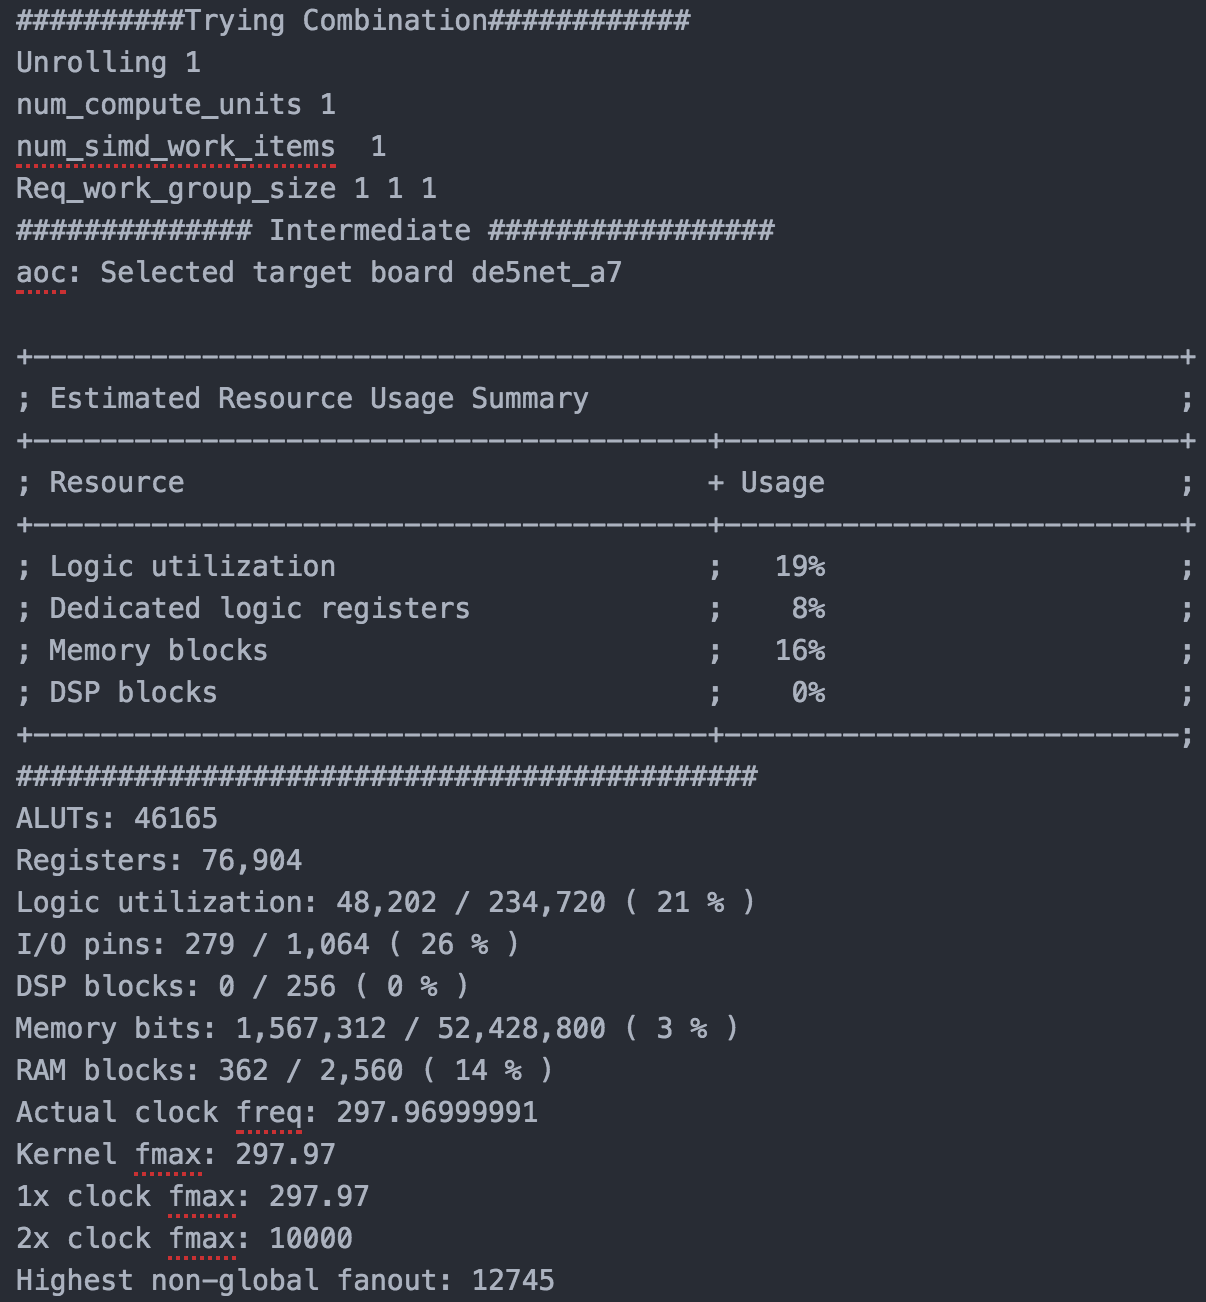
\includegraphics[scale=0.4]{sample_raw_data.png}
\caption{data set sample}
\label{figure:sample_raw_data}
\end{figure}

\section{Software Tools}
Python\citep{Rossum:1995:PRM:869369} is an object-oriented and interpreted programming language. It is one of the popular language for statistical analysis and machine learning. A large number of open source library are available for machine learning and plotting data. Here are some of the Python library used in this project.

\begin{enumerate}
    \item Matplotlib
        \begin{itemize}
            \item Matplotlib \citep{Hunter:2007} is a 2D plotting library written in Python and it produces produces figures in a variety of formats to be used in publications.
        \end{itemize}
    \item NumPy
        \begin{itemize}
            \item NumPy \citep{developersnumpy} is an extension to the Python programming language to support large, multi-dimension arrays and matrices.
        \end{itemize}
    \item Scikit-learn
        \begin{itemize}
            \item Scikit-learn \citep{scikit-learn} is an open source machine learning library written in Python. It features a variety of classification, regression and clustering algorithms. It is designed to interoperate with numerical library, NumPy and scientific library, SciPy.
        \end{itemize}
\end{enumerate}

\section{Classification Performance Metric}
Performance of the machine learning could be measured by using various metrics. In this project, we wanted to minimize false positive rate (FPR) and maximize true positive rate (TPR). Area Under the Receiver Operating Characteristic curve (AUC) takes both TPR and FPR into account. Therefore, AUC is chosen as the metric to measure the classification performance in this report.